\chapter{Serviceorientierte Architektur und Microservices}
Das folgende Kapitel behandelt Microservices, ihre Vor- und Nachteile und die Abgrenzung zu serviceorientierten Architekturen, sowie die Unterschiede zu monolithischen Architekturen.
\section{Definition und Abgrenzung}
Im Folgenden wird die Definition von Microservices und die Abgrenzung zu serviceorientierten Architekturen beschrieben.

\subsection{Definition von Microservices}
Microservice-Architekturen sind ein Ansatz, um große Softwarearchitekturen in kleine, konsistente, voneinander klar abgegrenzte Services zu zerlegen. Diese Services sind isoliert und kommunizieren miteinander. \cite[Kapitel 1]{MicroservicesForJavaDevelopers}

Microservices werden typischerweise von kleinen Teams implementiert, gebaut und deployt. Diese kleinen Services sind so autonom, dass das Team, welches für den Service zuständig ist, die Implementierungsdetails ändern kann, ohne großen Einfluss auf das gesamte restliche System zu nehmen.
Jedes Team ist selbst für sein Service verantwortlich. Das Team muss für die Aufgabenstellung die richtige Technologie wählen, das Service deployen und managen und etwaige Fehler beheben.
Bei Microservice-Architekturen kann die Abgrenzung der verschiedenen Services ganz klar definiert werden. \cite[Kapitel 1]{MicroservicesForJavaDevelopers} Dies hilft, um \cite[Kapitel 1]{MicroservicesForJavaDevelopers}
\begin{enumerate}[ref=\textbf{Punkt \arabic*}]
	\item \label{SOA:Abgrenzung:logik} die Logik des Services einfach zu verstehen, ohne den Kontext der gesamten Applikation kennen zu müssen.
	\item \label{SOA:Abgrenzung:bauen} den Service schnell lokal bauen und ausführen zu können.
	\item \label{SOA:Abgrenzung:technologie} die richtige Technologie für ein Problem zu nützen.
	\item \label{SOA:Abgrenzung:testen} den Service einfach und schnell testen zu können, ohne die gesamte Applikation dabei hochfahren zu müssen.
	\item \label{SOA:Abgrenzung:release} schnellere Releasezeiten zu ermöglichen.
	\item \label{SOA:Abgrenzung:skalierung} schnellere horizontale Skalierung zu ermöglichen.
	\item \label{SOA:Abgrenzung:belastbarkeit} die Belastbarkeit des Systems zu verbessern.
\end{enumerate}

Die oben angeführten Punkte werden im Folgenden näher ausgeführt \cite[Kapitel 1]{MicroservicesForJavaDevelopers}:

\ref{SOA:Abgrenzung:logik}: Jedes einzelne Microservice sollte nur einen Teil der gesamten Anwendung ausmachen. Ein Microservice deckt meist nur einen Geschäftsfall der gesamten Businesslogik ab. Dieser Geschäftsfall ist für sich einfacher zu verstehen, als das gesamte System. Kommt ein neuer Entwickler in das Team, muss er sich nur in den Code des Microservice, an dem er arbeitet, einlesen und muss nicht das gesamte System verstehen.

\ref{SOA:Abgrenzung:bauen}: Muss bei einem neuen Feature die gesamte Anwendung gebaut, deployt und ausgeführt werden, ist dies sehr aufwändig und kostet sehr viel Zeit. Ein Microservice hingegen steht für sich selbst und kann einfach lokal gestartet und getestet werden. Dies erleichtert dem Entwickler die Arbeit und spart Zeit.

\ref{SOA:Abgrenzung:technologie}: Meist werden für bestimmte Geschäftsfälle verschiedene Technologien benötigt. Ist die gesamte Businesslogik in einem Monolithen abgebildet, kann lediglich eine Technologie eingesetzt werden. Ist aber z.B. für einen bestimmten Geschäftsfall Machine Learning nötig, ist wahrscheinlich Java die falsche Lösung und man setzt lieber auf Python.
Microservices sind unabhängig voneinander und kommunizieren meist durch REST oder SOAP miteinander. Dadurch kann in jedem Service die gewünschte Technologie eingesetzt werden.

\ref{SOA:Abgrenzung:testen}: Ähnlich zu \ref{SOA:Abgrenzung:bauen}, wo das Bauen und Ausführen eines Microservice beschrieben wird, kann ein Service auch unabhängig vom gesamten System getestet werden.

\ref{SOA:Abgrenzung:release}: Heutzutage müssen neue Features schnell ausgeliefert werden, ansonsten ist womöglich der Konkurrent schneller und man verliert Kunden. Muss bei einem neuen Release das gesamte System neu deployt werden, sind damit verschiedenste Risiken verbunden. Wird z.B. ein fehlerhafter Code deployt, stürzt der gesamte Monolith ab. Bei Microservices ist in dieser Zeit lediglich das neu deployte Service nicht verfügbar.

\ref{SOA:Abgrenzung:skalierung}: Hat man ein monolithisches System und möchte einen neuen Geschäftsfall implementieren, muss dieser in das bestehende System eingeflochten werden, was dazu führen kann, dass ein bestehender Code nicht mehr so funktioniert wie gewollt.
Bei einer Microservice-Architektur wird ein neues Service für diesen Geschäftsfall angelegt und bestehender Code nicht oder kaum für Aufrufe des neuen Service geändert.

\ref{SOA:Abgrenzung:belastbarkeit}: Fällt ein Service aus, heißt das nicht, dass das gesamte System nicht mehr verfügbar ist. Teile des Systems können meist ohne Probleme weiterverwendet werden.



\subsection{Abgrenzung serviceorientierter Architekturen und Microservices}
Microservices und serviceorientierte Architekturen gehören beide zu den service-basierten Architekturen. Das heißt, dass beide Architekturen einen großen Schwerpunkt auf Services als primäre Architekturkomponenten legen. Obwohl Microservices und serviceorientierte Architekturen sehr unterschiedliche Muster aufweisen, haben sie auch vieles gemeinsam \cite[Kapitel 1]{MicroservicesVSSOA}.

Alle serviceorientierten Architekturen sind verteilte Architekturen. Die Servicekomponenten werden über Remote-Protokolle, wie z.B. Representational State Transfer (REST), Simple Object Access Protocol (SOAP) oder Java Message Service (JMS), angesprochen.
Beide bieten viele Vorteile im Vergleich zu monolithischen und schichten-basierten Architekturen. Sie bieten höhere Skalierbarkeit, losere Kopplung zwischen den Services und bessere Kontrolle über die Entwicklung, Tests und das Deployment. Komponenten in einer verteilten Anwendung tendieren mehr dazu in sich verschlossen zu sein und bieten daher besseres Änderungsmanagement und einfachere Wartung, was zu mehr Flexibilität und zu robusteren Anwendungen führt.
Diese Architekturen führen auch zu loser gekoppelten und modulareren Anwendungen. 
Modularität ist das Kapseln einzelner Teile der Anwendung in abgeschlossene Services, die dadurch individuell designed, entwickelt, getestet und deployt werden können, ohne großen Einfluss auf andere Services zu nehmen \cite[Kapitel 1]{MicroservicesVSSOA}.

Sowohl bei Microservices, als auch bei serviceorientierten Architekturen müssen \textit{Service Contracts} getroffen werden. Service Contracts werden zwischen einem Service und einem Servicekonsument (Client) vereinbart. Dadurch wird das Format der eingehenden und ausgehenden Daten spezifiziert (z.B. XML, JavaScript Object Notation [JSON], Java Object, etc.) \cite[Kapitel 1]{MicroservicesVSSOA}. 

Microservice-Teams bestehen meist aus maximal fünf bis sieben Personen. Das Team muss die Entwicklung, das Deployment und den Betrieb des Service alleine bewältigen. Je größer das Team, desto höher ist der Kommunikationsaufwand. Jedes Teammitglied sollte die gesamte Codebasis überblicken und warten können. Zu große Teams sind meist ausschlaggebend dafür, dass das Service aufgesplittet werden sollte \cite[Kapitel 2]{MicroservicesVSSOA}.

Serviceorientierte Architekturen sind eher für große, komplexe Enterprise-Systeme geeignet, die eine Interaktion mit vielen heterogenen Applikationen und Services benötigen. Für Anwendungen, die viele Komponenten benötigen und von mehreren Services geteilt werden, sind serviceorientierte Architekturen passender.
Für Applikationen mit einem wohldefinierten Arbeitsablauf und wenig gemeinsam geteilten Komponenten, wie z.B. Security-Komponenten, sind Microservice-Architekturen sinnvoll.
Microservice-Architekturen sind besser geeignet für kleine, wohl definierte web-basierte Systeme, wie für groß skalierbare Enterprise-Systeme. Die fehlende Middleware ist ein Faktor, weshalb Microservice-Architekturen nicht oder schlecht für komplexe Businessanwendungen geeignet sind. Microservices sollten dort eingesetzt werden, wo sich die Businesslogik auf kleine abstrahierte Geschäftsfälle herunterbrechen lässt \cite[Kapitel 2]{MicroservicesVSSOA}.

\begin{figure}[H]
	\begin{center}
		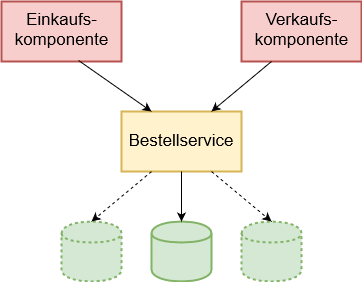
\includegraphics[scale=0.80]{SOA_Bestellservice.png}
		\caption[Serviceorientierte Architektur - Bestellservice]{Serviceorientierte Architektur - Bestellservice}
		\cite[Kapitel 3]{MicroservicesVSSOA}
		\label{fig:SOA_Bestellservice}
	\end{center}
\end{figure}

Microservices und serviceorientierte Architekturen sind auch bezüglich Teilen von Komponenten sehr unterschiedlich. Serviceorientierte Architekturen basieren auf dem Prinzip \textit{share-as-much-as-possible}, wohingegen Microservices auf dem Prinzip \textit{share-as-little-as-possible} basieren.
Angenommen ein großes Warenhaus benötigt zum Verwalten der Einkäufe und Verkäufe jeweils ein \textit{Bestell-Service}. Bei serviceorientierten Architekturen, wie in Abbildung \ref{fig:SOA_Bestellservice} zu sehen, würde man dazu das Bestell-Service einmal implementieren und die Einkaufs- und Verkaufskomponente teilen sich dieses Service. Das Bestell-Service selbst muss in diesem Fall wissen, welche Aktionen es bei den verschiedenen Anfragen ausführen muss.
Obwohl das \textit{share-as-much-as-possible}-Prinzip das Problem der Codeduplizierung löst, ist damit eine enge Kopplung von Businesskomponenten verbunden und erhöht das Risiko von Änderungen. Angenommen man ändert den Code im Business-Service, ist diese Änderung schwer zu testen, da das Service global verfügbar ist und je nach Aufruf andere Aktionen auslöst \cite[Kapitel 3]{MicroservicesVSSOA}.

Microservices basieren auf dem Konzept des \textit{share-as-little-as-possible} und verstärken dadurch das domain-driven Design Konzept \textit{Bounded Context}. Microservices sind lose gekoppelt und agieren daher als einzelne geschlossene Einheit mit wenig Abhängigkeiten. Es gibt lediglich ein wohldefiniertes Interface und wohldefinierte Vereinbarungen nach außen. 
Realistischerweise wird es immer gemeinsam geteilte Services geben, auch in Microservice-Architekturen, z.B. Sicherheits- oder Infrastrukturservices. Serviceorientierte Architekturen maximieren das Teilen von Komponenten, wohingegen Microservice-Architekturen dieses durch den klar definierten Bounded Context minimieren \cite[Kapitel 3]{MicroservicesVSSOA}.

Es gibt viele Vorteile, die das Verstärken des Bounded Context bringt. Die Wartung der Services wird wegen der geringeren Abhängigkeiten weitaus einfacher. Dies erleichtert auch das Ändern und Weiterentwickeln des Service. Auch das Deployment gestaltet sich dadurch um einiges einfacher, da weniger Code zu deployen ist und es weniger Risiken gibt, andere Bereiche des gesamten Systems zu brechen. Dies fördert auch die Robustheit des gesamten Systems \cite[Kapitel 4]{MicroservicesVSSOA}.


\section{Vergleich zu monolithischer Architektur}
Microservices und Monolithen sind sehr unterschiedliche Designstrategien, um eine Anwendung zu entwickeln. Beide Strategien haben ihre Vor- und Nachteile. Die Strategie sollte deshalb mit Bedacht gewählt werden. Die monolithische Architektur ist derzeit noch der Standardweg eine Applikation zu entwickeln \cite{FowlerDSM}.

Im Folgenden werden die wichtigsten Unterschiede monolithischer und Microservice-Architekturen beschrieben \cite[Kapitel 3]{MonolithVSMicroservices}

\subsection{Wartung}
Microservices sind viel einfacher zu warten, da sich die Komplexität eines Services in Grenzen hält. Microservices sind modulare und unabhängige Services. Neue Entwickler können sich in die Codebasis schneller einlesen und schneller neue Features implementieren, als bei monolithischen Architekturen.

Ein Monolith besteht aus einer Codebasis, wo alle Geschäftsfälle abgedeckt sind. Wird ein neues Feature hinzugefügt, wird es dabei in die bestehende Codebasis eingewebt. 
Dies erhöht die Komplexität des Codes und erschwert die Entwicklung und Wartung.
Neue Entwickler müssen sich in die gesamte Codebasis und in den gesamten Workflow einlesen, um neue Features entwickeln zu können.

\subsection{Deployment}
Ein kontinuierliches Deployment gestaltet sich bei Monolithen sehr schwierig, da der Monolith immer größer und komplexer wird. Zudem muss immer der gesamte Monolith deployt werden, auch wenn lediglich wenig Codestücke geändert wurden. Dies ist natürlich sehr zeitaufwändig, aber auch gefährlich. Wird ein fehlerhafter Code deployt, bringt dieser den gesamten Monolith zum Stillstand.

Bei Microservices hingegen wird die Codebasis in kleine, überschaubare Services unterteilt, die einzeln und jederzeit schnell deployt werden können. Wird bei Microservice-Architekturen ein fehlerhafter Code deployt, ist es möglich, dass andere Teile des gesamten Systems noch ohne Probleme laufen.

\subsection{Tests}
Auch beim Testen eines Monolithen werden die große Codebasis und die vielen verschiedenen Anwendungsfälle zum Problem. Das Testen aller Szenarien bei einer derart großen Codebasis wird dabei schnell unübersichtlich.

Bei Microservices kann durch den Bounded Context jede Komponente individuell getestet werden. Dies erleichtert das Testen eines jeden Services ungemein und verringert dazu auch die Fehleranfälligkeit eines Systems.

\subsection{Startup-Zeit}
Bei monolithischen Architekturen wird der gesamte Monolith hochgefahren. Je komplexer und größer dieser wird, desto mehr steigt die Startzeit.

Die Startzeit bei Microservices ist viel schneller, da jedes Service einzeln hochgefahren werden kann. Werden alle Services gemeinsam gestartet, bringt dies bezüglich der Startzeit wieder wenig.

\subsection{Technologie}
Ein Monolith wird in einer Programmiersprache entwickelt und greift meist nur auf eine Datenbank zu. Neue Technologien können nicht, bzw. nur sehr umständlich hinzugefügt werden. Die Einarbeitungszeit gestaltet sich jedoch bezüglich Technologie einfacher, da nur eine Sprache zum Einsatz kommt und neue Entwickler nur diese beherrschen müssen.

Mit Microservices können Entwickler die Technologie jedes Services selbst wählen. Die Services greifen oft auch auf verschiedene Datenbanken zu und Entwickler können auch die Wahl der Datenbank selbst wählen. Da Microservices so klein und überschaubar sind, können diese schnell ersetzt werden und es kann dadurch immer die aktuellste Version oder Technologie verwendet werden.

\subsection{Skalierbarkeit}
Microservices können einfach skaliert werden. Platform as a Service Plattformen, wie OpenShift, bieten eine einfache Möglichkeit, Services je nach Bedarf hoch- und runterskalieren zu können.

Einen komplexen Monolithen zu skalieren, gestaltet sich sehr schwierig. Zum Beispiel wird ein kontinuierliches Deployment mit vielen Entwicklern und einer sehr großen Codebasis sehr kompliziert.


\section{Charakteristiken}
Im Folgenden werden einige Charakteristiken von Microservices beschrieben, die auch für serviceorientierte Architekturen gelten \cite{SpringMicroservices}:

\subsection{Service-Vereinbarung}
Microservices werden durch wohldefinierte Service-Vereinbarungen beschrieben. Zum Datenaustausch kann z.B. REST oder SOAP verwendet werden. Als Markup-Sprache kann JSON, XML oder auch YAML eingesetzt werden. In der Welt der Microservices wird meist die Kombination von REST und JSON eingesetzt. Es gibt aber mehrere Möglichkeiten zur Definition von Service-Kontrakten. JSON Schema, WADL, Swagger und RAML sind nur ein paar wenige Beispiele.

\subsection{Lose Kopplung}
Microservices sind unabhängig und lose gekoppelt. Meist akzeptieren Microservices ein Event als Input und reagieren darauf erneut mit einem Event. Nachrichten, HTTP und REST werden häufig zur Interaktion zwischen den einzelnen Services eingesetzt. Nachrichten-basierte Endpunkte bieten dabei ein höheres Level an Entkopplung.

\subsection{Service-Abstraktion}
Service-Abstraktion bei Microservices ist nicht nur die abstrahierte Realisierung des Service, sondern bietet auch eine komplette Abstraktion von allen Bibliotheken und Umgebungsdetails.

\subsection{Wiederverwendung}
Microservices sind wiederverwendbare Business-Services. Sie werden von mobilen Geräten, Desktop-Anwendungen und auch anderen Microservices verwendet.

\subsection{Zustandslosigkeit}
Wohl-designte Microservices sind zustandslos und teilen sich nichts. Wird ein gemeinsamer Zustand in verschiedenen Services benötigt, wird dieser meist in einer Datenbank abgebildet.

\subsection{Interoperabilität}
Services sind durch Standardprotokolle und Nachrichtenaustausch-Standards interoperabel. Nachrichtenaustausch, HTTP und REST werden zum Nachrichtentransport verwendet. Eine Kombination aus REST und JSON ist die populärste Methode zum Entwickeln von interoperablen Services. Wird weitere Optimierung benötigt, kommen auch andere Protokolle, wie RabbitMQ, Avro, Zero MQ oder Protocol Buffers zum Einsatz. Der Einsatz dieser Protokolle kann dabei aber auch die Interoperabilität der Services einschränken.

\subsection{Zusammensetzung}
Microservices sind zusammensetzbar. Dies wird durch Service Orchestrierung und Service Choreografie erreicht. Service Orchestrierung und Service Choreografie sind zwei Designvarianten von Microservices. Auf diese wird im nächsten Abschnitt näher eingegangen.

\section{Varianten}
Im Folgenden werden die beiden Varianten \textit{Service Orchestrierung} und \textit{Service Choreografie} zum Design von Microservices vorgestellt.

\subsection{Service Orchestrierung}
Bei der Service Orchestrierung gibt es ein zentrales Kompositionsservice, dass das entsprechende Microservice aufruft und von diesem die Antwort erwartet. Diese Nachrichten können mittels HTTP oder Socketaufrufen durchgeführt werden. Wichtig hier ist, dass dieses Muster sowohl synchron, als auch asynchron durchgeführt werden kann. Das aufgerufene Microservice muss also nicht sofort antworten, sondern kann auch später mit der Antwort ein Event im Kompositionsservice auslösen.
In diesem Muster reden die Microservices nicht miteinander, sondern nur mit dem Kompositionsservice. Dabei muss jedoch nicht zu jedem Microservice dasselbe Protokoll verwendet werden, z.B. redet das Kompositionsservice mit Service A über HTTP und mit Service B über das XML/RPC Protokoll \cite[Kapitel 3]{PracticalMicroservices}.

Wie in Abbildung \ref{fig:SOA_Orchestrierung} zu sehen, wird dabei das Kompositionsservice zur zentralen Autorität. Hier beginnt auch die gesamte Logik, was schlechtes Design für Microservices bedeutet. Die gesamte Logik im Kompositionsservice zu haben, führt zu einer Fülle von Abhängigkeiten zwischen den Services, z.B. kann die Logik sein, dass wenn Service A antwortet, Service B danach aufgerufen werden muss. Dies führt zu Abhängigkeiten zwischen Service A und Service B \cite[Kapitel 3]{PracticalMicroservices}.

Da das Kompositionsservice der zentrale Punkt der Anwendung ist, ist dieser auch die Schwachstelle. Dieses Service muss verfügbar sein, ansonsten steht die gesamte Anwendung still. Das Kompositionsservice ist der \textit{Single-Point-of-Failure} in dieser Architektur. Dies kann aber durch Tools und cloud-basierte Lösungen, wie Skalieren oder Clustering gelöst werden. Zusätzlich ist das Orchestrierungsmuster schwer zu implementieren. Hat man einen Entscheidungspunkt, wird es schwer, dem verteilten Design zu folgen \cite[Kapitel 3]{PracticalMicroservices}.

\begin{figure}[H]
	\begin{center}
		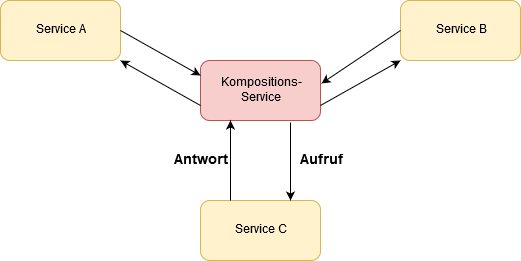
\includegraphics[scale=0.8]{SOA_Orchestration.png}
		\caption[Varianten - Service Orchestrierung]{Varianten - Service Orchestrierung}
		\cite[Kapitel 3]{PracticalMicroservices}
		\label{fig:SOA_Orchestrierung}
	\end{center}
\end{figure}

\subsection{Service Choreografie}
Anders als bei der Service Orchestrierung, ist bei der Service Choreographie jedes Service in Koordination mit den anderen Services auf einen bestimmten Anwendungsfall zugeschnitten.
Service Orchestrierung repräsentiert die Kontrolle von einem einzelnen Standpunkt aus. Bei der Choreografie wird jedes Service in die Interaktion mit eingebunden \cite[Kapitel 3]{PracticalMicroservices}. 

Wie in Abbildung \ref{fig:SOA_Choreographie} zu sehen, redet bei der Service Choreografie jedes Service nach Abschluss des Tasks mit einem anderen Service, um die nächste Aufgabe zu triggern. Dies kann in den Mustern \textit{one-to-one}, \textit{one-to-many} oder \textit{many-to-many} geschehen. Dies kann ebenfalls synchron oder asynchron durchgeführt werden. Idealerweise gibt es ein globales Protokoll, über das die Services miteinander kommunizieren. Meistens werden diese Aufrufe asynchron durchgeführt. Da es kein zentrales Service gibt, löst jedes Service ein Event nach Abschluss seines Tasks aus. Dies macht die Services unabhängig von einander und fördert die lose Kopplung. Andere Services registrieren sich auf dieses Event und reagieren darauf, wenn es ausgelöst wird \cite[Kapitel 3]{PracticalMicroservices}. 

Durch nachrichtenorientierte Kommunikation kann das Choreografiemuster sehr nützlich werden. Zwischen den Services wird eine Nachrichtenschlange implementiert. Dadurch wird das Loslösen, Hinzufügen und Entfernen von Services sehr einfach gelöst. Auch die ganze Reihe an Abhängigkeiten, die oft bei Choreografiemustern entstehen, wird dadurch gelöst. Service Choreografie erhöht die Komplexität eines Systems. Jedes Service erzeugt und verarbeitet Nachrichten zur Laufzeit. Dadurch kann der exakte Stand einer Transaktion nicht herausgefunden werden \cite[Kapitel 3]{PracticalMicroservices}.

\begin{figure}[H]
	\begin{center}
		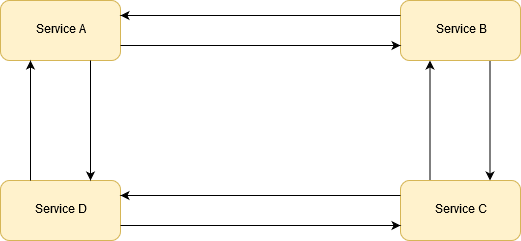
\includegraphics[scale=0.8]{SOA_Choreographie.png}
		\caption[Varianten - Service Choreografie]{Varianten - Service Choreografie}
		\cite[Kapitel 3]{PracticalMicroservices}
		\label{fig:SOA_Choreographie}
	\end{center}
\end{figure}

\section{Vor- und Nachteile}
Im folgenden Abschnitt werden die Vor- und Nachteile von Microservices behandelt.

\subsection{Vorteile}
\subsubsection{Technologieunabhängigkeit}
Microservices werden als eigenständige Einheit betrachtet. Dadurch können die einzelnen Services verschiedene Technologien verwenden. Greift ein Service auf eine Datenbank zu und ein anderes Service führt Shell-Skripte aus, beeinflussen sich die beiden Services nicht und können jederzeit ausgetauscht werden, ohne Einfluss auf andere Services zu nehmen. Performance ist in diesem Zusammenhang ebenfalls sehr wichtig. Wird eine Technologie zu langsam, kann sie ohne Probleme durch eine neue ersetzt werden \cite[Kapitel 1]{Newman2015}.

\subsubsection{Skalierung}
Wie erwähnt, muss bei Monolithen die gesamte Software als Ganzes deployt und skaliert werden. Dies bedeutet viel Overhead. Bei Microservices können einzelne Teile hoch- und runterskaliert werden. Cloud-basierte Technologien, wie z.B. OpenShift, bieten diese Möglichkeit an. Es kann aber auch ein Microservice auf einer besseren Hardware laufen. Die anderen Services bleiben auf der billigeren Hardware. Monolithen müssten als Ganzes auf der besseren Hardware laufen. Dies verringert die Kosten der Skalierung bei Microservices drastisch \cite[Kapitel 1]{Newman2015}.

\subsubsection{Austauschbarkeit}
Bei Microservices ist es sehr einfach, den bestehenden Code zu ändern oder auszutauschen. Da diese unabhängig sind, sind keine anderen Teile des Systems betroffen. Bei Monolithen stellt dies oft ein großes Risiko dar. Der Code ist oft sehr verwoben und kleine Änderungen haben große Auswirkungen \cite[Kapitel 1]{Newman2015}.

\subsubsection{Entwicklerteam}
Entwickler greifen bei monolithischen Architekturen oft auf die selben Teile des Codes zu. Bei Versionierungsprogrammen, wie GIT oder Subversion, führt dies oft zu Konflikten.
Microservices können getrennt voneinander bearbeitet und der Code ohne Probleme zusammengefügt werden \cite[Kapitel 1]{Newman2015}.


\subsection{Nachteile}
\subsubsection{Hohe Latenzzeiten}
Microservices reden über das Netzwerk miteinander. Dieser Kommunikationsweg ist natürlich viel langsamer, als wenn diese in derselben JVM miteinander reden würden. Dies führt zu hohen Latenzzeiten. Diese müssen bei der Architektur von Microservices berücksichtigt werden \cite[Kapitel 1]{Newman2015}.

\subsubsection{Wiederverwendbarkeit von Code}
Microservices sind unabhängige und eigenständige Einheiten. Sie haben im besten Fall keine Abhängigkeiten zueinander. Dadurch verringert sich die Wiederverwendbarkeit von Code. Dies führt auch zu einer Codeverdopplung. Wird dasselbe Codestück in zwei verschiedenen Services benötigt, muss es in beiden vorhanden sein \cite[Kapitel 1]{Newman2015}.

\subsubsection{Deployment}
Jedes Service muss einzeln deployt werden. Dazu wird ein eigener Deployment-Prozess pro Service benötigt. Dies bedeutet Aufwand für den Entwickler und es muss eine eigene Infrastruktur geschaffen werden, was zusätzlich Kosten generiert \cite[Kapitel 1]{Newman2015}.
